\documentclass[letterpaper,twocolumn]{article}

\usepackage[top=1in,bottom=1in,left=0.75in,right=0.75in]{geometry}
\usepackage{graphicx}
\usepackage{newtxtext}
\usepackage{newtxmath}
\usepackage{pifont} % For checkmarks in tab:nat-matching.
\usepackage[hyphens]{url}
\usepackage[table]{xcolor}

\usepackage[textsize=footnotesize]{todonotes}\setlength{\marginparwidth}{1.5cm}

% Better look for citations that include a section reference like \cite[\S 3]{foobar}.
\usepackage{cite}
\renewcommand{\citemid}{~}

% Load hyperref after other packages.
\usepackage[pdfa,hidelinks,pdfcreator={},pdfproducer={}]{hyperref}
\urlstyle{same}
\def\sectionautorefname{Section}
\def\subsectionautorefname{Section}

% Disable metadata for reproducible PDF.
% https://tex.stackexchange.com/a/313605
\usepackage{ifpdf}
\ifpdf
\pdfinfoomitdate=1
\pdftrailerid{}
\pdfsuppressptexinfo=-1
\fi

\hyphenation{Web-RTC}
\hyphenation{Java-Script}
\hyphenation{uProxy}

% Highlight the first usage or definition of a technical term.
% Like the firstterm element in DocBook: https://tdg.docbook.org/tdg/5.2/firstterm.html.
\newcommand{\firstterm}[1]{\textit{#1}}

\begin{document}

\date{}

\title{Snowflake, a censorship circumvention system \\using temporary WebRTC proxies}

\author{}

\maketitle

\begin{abstract}
Snowflake is a system for circumventing Internet censorship.
It~derives its blocking resistance from
the use of numerous, ultra-light, temporary proxies (``snowflakes''),
which accept traffic from censored clients using peer-to-peer WebRTC protocols
and forward it to a centralized bridge,
which does the real work of directing traffic to its destination.
The temporary proxies are lightweight enough to be implemented in JavaScript,
in a web page or browser extension,
making them vastly cheaper to set up than
a traditional proxy or VPN server.
The proxies are not assumed to have stable network addresses
or be online all the time,
and even the blocking of currently in-use proxy
is not fatal to a circumvention session,
as the system permits clients to switch proxies on the fly.

% Need anything about broker, centralization here?

Snowflake has been deployed with success
in Tor Browser and Orbot for several years.
It has been significant for circumvention
during high-profile network disruptions,
including in Russia in~2021 and Iran in~2022.
In this paper, we explain the composition of Snowflake's many parts,
give a history of deployment and attempts to block~it,
and reflect on implications for circumvention generally.
\end{abstract}

% General references:
%   https://keroserene.net/snowflake/technical/#history
%   https://www.bamsoftware.com/papers/thesis/#chap:snowflake

\section{Introduction}
\label{sec:intro}

Censorship circumvention systems
may be characterized on multiple axes.
There are those that seek to avoid blocking
by imitating some common, high-value protocol;
and those that randomize their protocols
in order not to look like any other protocol in particular.
Some concentrate their traffic into one, or a few,
well-known proxies, somehow entangled with other traffic
such that a censor cannot easily block them;
and others that spread their traffic out over
hundreds or thousands of proxies,
none of which is individually difficult to block,
but which are difficult for a censor to discover and block in their entirety.
What all circumvention systems have in common
is that they strive to increase the \emph{cost}
to the censor of blocking them---whether that be
in the form of research and development,
human resources, and hardware,
or in the inevitable overblocking that results
when a censor tries to block circumvention traffic
that is difficult to distinguish from other traffic
the censor values highly.
On the spectrum of mimicry to randomization,
Snowflake falls more on the mimicry side;
on the scale of concentrated to diffuse,
it is diffuse.
If~Snowflake has a single distinguishing characteristic,
it is that it pushes this idea of distributed, disposable
proxies to an extreme,
by making proxies extremely cheap to run,
in web browsers, using WebRTC to communicate.

WebRTC is a suite of interacting protocols
intended to enable real-time communication applications
in web browsers~\cite{rfc8825}.
Video and voice chat are familiar and typical examples
of WebRTC applications.
Snowflake exchanges WebRTC data formats
in the course of establishing a connections,
and uses WebRTC protocols for NAT traversal
and for data transfer between the client and a temporary proxy.
Critically for Snowflake, WebRTC protocols
are exposed by JavaScript APIs in web browsers,
meaning it is possible to implement a WebRTC-based proxy
in an ordinary web page or browser extension.
WebRTC is also usable outside a browser,
which is how we implement the Snowflake client program
and alternative, command line--based proxies.

As is typical in circumvention research,
we assume a threat model where
censored \firstterm{clients} reside in a censor-controlled network.
The \firstterm{censor} has the power to inspect and interfere with
traffic that crosses the border of its network;
in practice, this power takes the form of things like
inspection of IP addresses and destination server hostnames,
dynamic protocol detection,
IP address blocking, and injection of false DNS responses
or TCP RST packets.
The client wants to exchange some information with a
destination outside the censor's network---often
with the assistance of third-party \firstterm{proxies}---and
the censor is motivated to block either the contents
of the communication, or the destination itself.
The censor is aware of the possibility of circumvention,
and therefore seeks not only to block direct access,
but also indirect access by way of a proxy or proxy protocol.
We consider circumvention to be accomplished when a client
can reliably reach any proxy,
because the proxy then provides access to any desired destination.
(In Snowflake, we separate the roles of temporary \firstterm{proxies}
and a stable long-term \firstterm{bridge}, but the idea is the same.)
Mitigating in the client's favor
is the fact that the censor is presumed to derive some benefit
from permitting some forms of network access:
the censor cannot trivially ``win''
simply by blocking all connections,
but must be selective in what to block and allow
in order to optimize some objective of its own.
The art of censorship circumvention is
forcing the censor into a difficult dilemma
of overblocking or underblocking,
by making circumvention traffic difficult to distinguish
from traffic that the censor finds valuable.

Snowflake has its origin in two earlier projects:
flash proxy and uProxy.
% https://lists.torproject.org/pipermail/tor-dev/2016-January/010310.html "Snowflake is a webrtc pluggable transport inspired by flashproxy."
% https://keroserene.net/snowflake/technical/#1-introduction "It is inspired by and builds upon the previous work of Flashproxy. Snowflake is much like a hybrid of previous Pluggable Transports..."
Flash proxy~\cite{Fifield2012a}, like Snowflake, used a model
of untrusted, temporary JavaScript proxies running in web browsers;
however the link between client and proxy was WebSocket
rather than WebRTC.
(WebSocket still finds use in Snowflake,
but only on the proxy--bridge link,
not the client--proxy link.)
Flash proxy was deployed in Tor Browser
% 2013: https://blog.torproject.org/combined-flash-proxy-pyobfsproxy-browser-bundles
% 2016: https://bugs.torproject.org/17428#note_2203210 "Remove Flashproxy from Tor Browser"
from 2013 to~2016,
but it never saw much use,
probably because the reliance on WebSocket,
which are TCP-based and do not have built-in NAT traversal like WebRTC does,
and required uses to perform a
% https://gitlab.torproject.org/legacy/trac/-/wikis/doc/PluggableTransports/FlashProxy/Howto
cumbersome port forwarding procedure.
WebRTC was at the time an emerging technology, and while
% https://bugs.torproject.org/5578 "Investigate WebRTC for flash proxy NAT punching "
% flashproxy.pdf §5.2: "New technologies like WebRTC [24] may fill this need in the future, if they become sufficiently popular that flash proxies' use of them does not stand out as unusual."
it was considered as a future transport protocol for flash proxy,
it was decided to begin Snowflake as a new, separate project,
rather than build atop flash proxy.
% https://serene.cx/snowflake/#note-flashproxy "...one could say that uProxy and flashproxy are the ancestors of snowflake."
uProxy~\cite{uproxy}, in one of its early incarnations,
% "in one of its earlier incarnations": uProxy pivoted from friend proxies to cloud servers in 2016:
%  https://web.archive.org/web/20161211194847/https://blog.uproxy.org/2016/02/get-access-24x7-through-your-own-uproxy.html
pioneered the use of WebRTC proxies.
uProxy's proxies were browser-based,
but the trust and deployment model was rather different
from flash proxy's and Snowflake's.
There was no centralized proxy discovery;
instead each censored client would arrange, out of band,
% uProxy v1.2.5 Design Doc: https://docs.google.com/document/d/1t_30vX7RcrEGuWwcg0Jub-HiNI0Ko3kBOyqXgrQN3Kw
% "uProxy depends on leveraging existing trust relationships to to find and use a proxy."
for a personal acquaintance, outside the censor's network,
to run a proxy in their web browser.
The social trust relationship was necessary to prevent misuse,
because the browser proxies fetched destination content directly,
without any further intermediary like the bridge in Snowflake.
A~uProxy proxy was expected to be
persistent and always online;
clients did not changes proxies on the fly.
% https://github.com/uProxy/uproxy-obfuscators
uProxy supported protocol obfuscation:
though the communication protocol was fundamentally WebRTC,
the contents of packets could be transformed so as not to resemble WebRTC.
This was possible because uProxy ran as a privileged browser extension
with access to socket operations.
Since Snowflake uses ordinary unprivileged browser APIs,
its WebRTC is restricted to looking like WebRTC;
on the other hand, because of that,
it is even easier to deploy a Snowflake proxy.
Like flash proxy, uProxy was active in the years
% 2013: Serene's 30C3 lightning talk on uProxy https://events.ccc.de/congress/2013/wiki/Static:Lightning_Talks#Day_3
2013--2016\todo{Check 2016 end date for uProxy}.

The closest existing system to Snowflake is MassBrowser~\cite{Nasr2020a}.
% https://github.com/net4people/bbs/issues/32
It incorporates many circumvention techniques, one of which is
proxying though volunteer proxies, called buddies.
The architecture is similar to Snowflake's:
there is a centralized component responsible for coordinating
connections between clients and proxies called the operator,
like Snowflake's broker;
MassBrowser buddies correspond to our snowflake proxies.
The trust model is intermediate between those of Snowflake and uProxy:
buddies may provide proxy service to strangers and not only their social acquaintances,
but buddies specify categories of content they are willing to directly proxy,
in order to mitigate misuse.
Buddies preferentially operate as one-hop proxies,
but also support proxying into a Tor bridge, as in Snowflake;
this option, however, is treated as a last resort rather than a default mode,
in keeping with MassBrowser's guiding principle of
of prioritizing blocking resistance and performance
over anonymity and privacy.
An~innovation in MassBrowser not present in Snowflake is client-to-client proxying:
clients may act as buddies for other clients,
with the reasoning that what is censored for one client may not be censored for another.
The buddy software is standalone application software,
which means that it, like uProxy, can use protocol obfuscation
% V-D: "We also implement traffic obfuscation to protect MassBrowser's traffic
% against traffic analysis attacks. Particularly, we have built a custom
% implementation of the obfsproxy Tor pluggable transport tailored to work with
% our MassBrowser implementation."
% VI-A: "MassBrowser uses a custom protocol over TCP/UDP for the communications
% between Clients and Buddies."
on the client--buddy link.
Like Snowflake, MassBrowser has been deployed to real users
and tested in practice against censors.
Protozoa~\cite{Barradas2020a}
% https://github.com/net4people/bbs/issues/55
is superficially similar
to Snowflake in its use of WebRTC,
but the two systems are essentially different.
More like uProxy, Protozoa has a one-to-one proxy model:
client and proxy discover one another and arrange a connection out of band,
and the proxy persists as long as the client is using it.
If Snowflake's specialty is diversity of proxy addresses,
Protozoa's is traffic analysis:
using an authentic WebRTC audio or video stream as a carrier,
it replaces the content of encrypted, encoded media frames
with covert ciphertexts of the same length,
such that the replacement is undetectable to an observer.
One technical subtlety is that where Snowflake uses
WebRTC data channels,
Protozoa uses WebRTC media streams,
which may be an advantage;
we will return to this point in \autoref{sec:fingerprinting}.
\todo{Check if \href{https://censorbib.nymity.ch/\#Figueira2022a}{Stegozoa}
and \href{https://censorbib.nymity.ch/\#Barradas2020b}{CRON} are relevant,
and discuss if so.}

% Very early versions of Lantern (circa 2014) used social network–based trusted proxies:
%   https://web.archive.org/web/20140326223853/http://techpresident.com/news/wegov/24455/why-remarkably-similar-circumvention-tools-uproxy-and-lantern-are-not-overkill
%   https://lists.torproject.org/pipermail/tor-dev/2014-March/006356.html "HOWTO use Lantern as a pluggable transport"
%   https://web.archive.org/web/20130831160152/https://www.youtube.com/watch?v=aiPkCugE-RY
%   https://web.archive.org/web/2oe_/http://wayback-fakeurl.archive.org/yt/aiPkCugE-RY
% But it wasn't WebRTC, so was less like Snowflake than uProxy was.
% I'll draw the line here, since even Tor bridges are "volunteer-operated" in a sense.

There is a tendency in writing about
circumvention research to disproportionately emphasize
the deficiencies of other systems
and the advantages of one's own.
It may give an impression to the reader
that the state of censorship circumvention
is more dire than it really is.
Such is not our aim.
While challenges remain,
today's circumvention systems are largely successful
and work in the situations people need them to.
For many people, circumvention is just another part of their
day-to-day use of the Internet.
With Snowflake, we are exploring a different point in the design space,
one with a different set of tradeoffs of advantages and disadvantages,
but not categorically superior in every dimension.
Here we present not only the design of Snowflake
and the principles that explain why it should be hard to block,
but also the experience of deployment on a large scale.
A~great deal of the interest in this kind of research
is in the complications that emerge when idea meets practice.

\todo{Origin of the name Snowflake?}
\todo{Deployed since\ldots}

\section{How it works}
\label{sec:mechanics}

\begin{figure*}
\framebox[\textwidth]{\vbox to 2in{\vfil\centering TODO\vfil}}
\caption{
Architecture of Snowflake.
}
\label{fig:architecture}
\end{figure*}

A~Snowflake proxy connection proceeds in three phases.
First, there is the rendezvous, where a client
signals its need for circumvention service
and is matched with a temporary proxy.
Then, there is connection establishment,
where the client and its temporary proxy connect to one another
with WebRTC, using information exchanged during rendezvous.
Finally, there is data transfer,
where the proxy ferries data back and forth
between the client and a remote service
(e.g., a Tor bridge).
\autoref{fig:architecture}
illustrates the process.

The client's circumvention session
does not begin and end with any particular temporary proxy.
Rather, the client strings together
a series of proxies, switching to a new one
whenever an old one goes offline.
This proxy handoff is hidden from the upper-layer protocols
(i.e., the web browser) that use the circumvention tunnel:
to them the Snowflake session appears as one long unbroken connection.

There is an ambient population of temporary Snowflake proxies.
For the most part, these proxies are the web browsers of people who have
installed the Snowflake proxy WebExtension,
or a functionally equivalent headless command-line version.
The proxies periodically poll a centralized server, the broker,
to inquire whether there are any clients that need service.
The broker is responsible for matching and
keeping track of associations between clients and proxies.

A~client begins a Snowflake session by
sending a rendezvous message to the broker.
The rendezvous message must be sent over a blocking-resistant channel,
which may however be slow or expensive; see \autoref{sec:rendezvous} for some examples.
When a client rendezvous message arrives,
the broker chooses one of the immediately available proxies,
subject to NAT compatibility and other matching criteria,\todo{Are there other matching criteria?}
forwards the client's rendezvous message to that proxy,
and conveys the client's downstream answer to the rendezvous back to the client.
The client and proxy then initiate a WebRTC connection
with each other; the broker is no longer involved.
Further details on rendezvous will be presented in \autoref{sec:rendezvous}.

The temporary proxy connects both to its assigned client
and to a centralized bridge,
and begins to copy bytes between the client and the bridge
in both directions.
Details about how the connections are established are in \autoref{sec:ice}.
This continues until the client ends its session by disconnecting,
or the proxy goes offline
(which happens, for example, when the web browser where a proxy is running is closed).
When a proxy goes offline,
it does not spell the end of the client's session:
the client and the bridge share end-to-end session state
that persists beyond the lifetime of any single proxy.
The client sends another rendezvous message to the broker,
is assigned another proxy,
and picks up where it left off.
More information about the data transfer phase is in \autoref{sec:data-transfer}.

Never does the client communicate with the broker or bridge directly.
Both the broker and the bridge may be blocked,
from the perspective of the client.
The client only communicates with the broker over an indirect rendezvous channel
that is assumed to be difficult and expensive for a censor to block.
The client only communicates with the bridge via a temporary proxy.
No single temporary proxy is critical to the operation of the system.
A~proxy may be blocked---even while it is in active use by a client---and
clients can adapt by using a different proxy.

\subsection{Rendezvous}
\label{sec:rendezvous}

In the first phase of establishing a Snowflake circumvention session,
the client exchanges a small amount of information with a server
outside the censor's zone of control,
in a process called rendezvous.
It is not possible for a Snowflake client
to establish a peer-to-peer WebRTC connection
with a temporary proxy straight away.
(For one thing, neither the client nor the proxy
know a network identifier for each other at the outset.)
The client and proxy bootstrap a connection between them
by way of a separate blocking-resistant channel
(i.e., something other than WebRTC)
and an intermediary known as the broker.

Rendezvous is not unique to Snowflake;
it is a fairly common component of circumvention designs.
Precedents include the
DEFIANCE Rendezvous Protocol~\cite[\S 3]{Lincoln2012a}
the facilitator interaction in flash proxy~\cite[\S 3]{Fifield2012a},
and the registration proxy in Conjure~\cite[\S 4.1]{Frolov2019b}.
Even commercial VPNs built on commodity protocols
often require contacting some kind of API server
before initiating a connection, which can also be considered rendezvous.
A~key property of rendezvous-using systems
is that they do not rely on any preshared secret information.
The client user needs only to acquire the necessary software;
whatever additional information is required to establish a circumvention session
is exchanged dynamically, at runtime.
A~corollary of the no-secret-information property
is that an adversary---the censor---has
no special disadvantage in attacking the system:
they may download the client software
and then act in every way as a normal user.
This is in contrast to other systems in which,
after acquiring the necessary circumvention software,
a~client must also get ahold of some secret,
such as a password or proxy address,
through an out-of-band channel
presumed to be unavailable to the censor---and
blocking resistance hinges on that secret information
remaining unknown to the censor.
In rendezvous-based systems like Snowflake,
if the censor does not block a proxy server,
it is not out of ignorance,
but because the censor is constrained in some other way,
for example by computational limitations
or fear of collateral blocking.

If rendezvous has the advantage of not requiring secrecy,
its disadvantage is that it presents one more thing to worry about.
Not only the main data transfer channel
but also the rendezvous channel must resist blocking:
the system as a whole is only as secure as the weaker of the two.
The saving grace here is that the security and performance requirements
of rendezvous are different, and generally more lenient.
Rendezvous can afford to be relatively more heavyweight,
slow, expensive, or inefficient for the sake of blocking resistance,
because it accounts for only a small fraction of the overall communication
and occurs only intermittently.
The enlarged design space of rendezvous encompasses
forms of data hiding that would be impractical
for bulk data transfer.
Another helpful consideration is that rendezvous protocols
are separable from the rest of the system.
The assumption of using WebRTC is embedded fairly deeply in Snowflake;
but the rendezvous part is modular,
not coupled to WebRTC or even any single other protocol.

Snowflake rendezvous requires a bidirectional exchange:
the client sends one message to the broker, then receives
one message in reply.
(This is a step backward from flash proxy,
which required only one outgoing message for its rendezvous,
but the communication model of WebRTC makes a reply message unavoidable.)
It is therefore a good fit for request--response protocols,
like those based on HTTP.
We currently support two rendezvous methods in Snowflake:

\begin{description}
\item[Domain fronting]
In this method, the client does one HTTPS exchange
with the broker; however routing through an intermediary such as a CDN
and disguising the externally visible domain name
(the TLS Server Name Indication, or SNI) so that the exchange
appears to be destined to a different site.
We defer to Fifield et~al.~\cite{Fifield2015a}
for a complete description of domain fronting.
\item[AMP cache]
% https://gitlab.torproject.org/tpo/anti-censorship/pluggable-transports/snowflake/-/merge_requests/50
AMP is a framework for web pages written in a restricted dialect of HTML.
Part of this framework is a free-to-use
cache server~\cite{amp-cache}.
Because the cache fetches upstream pages on demand,
it works as a specialized sort of HTTP proxy.
By encoding rendezvous messages as AMP-conformant HTML,
we can use the cache as a proxy for rendezvous,
one that is not easily blocked without blocking the cache server as a whole.
This rendezvous method still requires domain fronting,
because the AMP cache protocol would otherwise expose the
upstream server's domain name in the TLS SNI,
but it increases the number of usable intermediary nodes.
\end{description}

The rendezvous component is, however, modular,
and any system that can be persuaded to indirectly convey a request
of about 1500 bytes, and a response of about the same size,
can work as a plug-in rendezvous method.
% https://bugs.torproject.org/tpo/anti-censorship/pluggable-transports/snowflake/25594
For example, encrypted DNS
% https://bugs.torproject.org/tpo/anti-censorship/pluggable-transports/snowflake/25874
% \cite[\S 3.4]{Fifield2020a}
(DNS over TLS or DNS over HTTPS):
the client encodes its registration message as a series of DNS queries;
the broker acts as an authoritative resolver;
and a third-party recursive resolver acts as an indirect intermediary,
while DNS encryption hides the broker's domain name in queries
from external observers.
% Flash proxy email rendezvous would not work for Snowflake, because unidirectional.
% https://gitweb.torproject.org/flashproxy.git/tree/flashproxy-reg-email
% https://gitweb.torproject.org/flashproxy.git/tree/facilitator/fp-registrar-email

A~Snowflake rendezvous message is a serialized bundle of data.
Its essential element
is the information necessary to establish a WebRTC connection,
namely a Session Description Protocol (SDP) \firstterm{offer}~\cite{rfc8839}.
The offer contains information needed for a network connection,
such as the client's external IP addresses;
as well as cryptographic information to secure a later key exchange between the peers.
% Specifically, a certificate fingerprint: https://www.rfc-editor.org/rfc/rfc8122.html#section-5
The rendezvous message also contains the client's
self-measured NAT type, which the broker will use to try to match it
with a compatible proxy.
The client serializes all these pieces of data and sends them to the broker.
The broker chooses an available proxy
and forwards the client's offer to it.
The proxy composes an SDP \firstterm{answer},
containing its own external addresses and cryptographic information,
and sends it back to the broker,
which then forwards it to the client.
Having exchanged an offer and answer,
the client and proxy are now able to establish a direct WebRTC connection,
without the broker in the middle.
The gathering of external IP addresses
forms part of the ICE protocol
and uses third-party STUN servers,
\todo{Should say more about STUN and gathering of ICE candidates here.}
which are described in more detail in \autoref{sec:ice}.

In WebRTC terms, the offer/answer exchange is called
``signaling,'' and the broker here acts as a signaling server.
While signaling is a necessary component
of any WebRTC-based system,
there is no specified way of doing it.
Every application must invent its own signaling system
according to its requirements
(which for us include covertness and blocking resistance).
Because of the lack of uniformity in accomplishing signaling,
the way a WebRTC application does (or does not do) signaling
may be a distinguishing feature; see \autoref{sec:fingerprinting}
for more considerations along these lines.

\begin{figure}
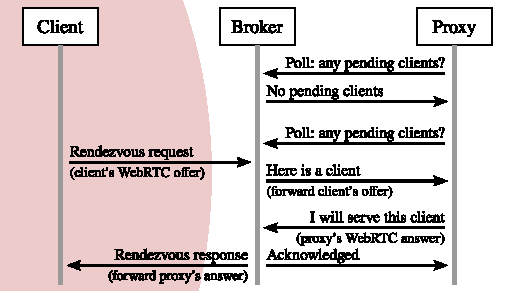
\includegraphics{figures/rendezvous/rendezvous}
\caption{
The long-polling communication model of Snowflake rendezvous.
The assigned proxy connects twice in between the time
the client sends its message and receives the response;
to the client it looks like one roundtrip.
Here, the client's rendezvous method is abstracted;
in reality the censor never contacts the broker directly,
but only via an intermediary.
The shaded background shows the censor's zone of control.
}
\label{fig:rendezvous}
\todo[inline]{Replace provisional graphic.}
\end{figure}

We use a ``long polling'' model for the client's side of broker interaction.
See \autoref{fig:rendezvous}.
There are proxies polling the broker constantly.
Each poll is an HTTPS request to a designated URL path.
(We assume there is no need for covertness
in the proxies' interaction with the broker,
because this side is outside the censor's observation and control.)
On receiving a poll request,
the broker does not send an HTTPS response immediately,
but waits for a few seconds to see if a client will become available.
If not, the broker sends a response saying ``no clients''
and the proxy sleeps for a while before trying again.
If a client rendezvous does arrive,
the broker extracts the SDP offer and forwards it to the proxy
in the HTTPS response.
The proxy computes its SDP answer,
then sends it back to the broker in a new HTTPS request
(with an attached identifier to permit the broker to match it
with the earlier polling request.)
Meanwhile, the client has been waiting for a response
to its rendezvous message.
The broker encapsulates the proxy's SDP answer
and sends it to the client over the rendezvous channel,
and simultaneously sends an acknowledgement to the proxy.
Now that the client and proxy have each other's
SDP information, they are ready to actually connect to one another.

\subsection{Peer-to-peer connection establishment}
\label{sec:ice}

After rendezvous,
a censored client in need of service
and a temporary snowflake proxy
will have exchanged
(among other information)
their IP addresses,
using the broker as an intermediary.
After this point, the broker is no longer involved
(as~far as that specific client--proxy pairing goes).
The next step is for the client and proxy
to establish a direct connection---which
is not a trivial operation,
even in the absence of censorship,
because of possible interference by
network address translation (NAT)
and ingress filters at either endpoint.
(Recall that many proxies run in web browsers
in ordinary residential ISPs,
without the connectivity of a typical Internet server.)
WebRTC is designed for exactly this use case
and has built-in facilities for traversing NAT.
Specifically, WebRTC uses
ICE (Interactive Connectivity Establishment)~\cite{rfc8445},
a procedure for testing candidate pairs of peer network addresses
until finding one that works.
ICE~makes use of
STUN (Session Traversal Utilities for NAT)~\cite{rfc8489}
and third-party STUN servers that provide services such as,
for example, allowing a network host to
discover its own external IP addresses.
In~Snowflake, candidate IP addresses are gathered
during rendezvous, with the assistance of STUN servers,
and sent as part of rendezvous messages.
ICE~may also use
TURN (Traversal Using Relays around NAT)~\cite{rfc8656},
effectively a UDP proxy.

There is no guarantee that two arbitrary peers will be able to make
a connection using the facilities of STUN alone.
Some mapping and
filtering setups are simply incompatible with one other.
Most uses of ICE would fall back to TURN in this case,
inserting a relay server between the peers to resolve any difficulties.
TURN is problematic for Snowflake,
because TURN relays' IP addresses are
generally fixed and easily discoverable by a censor.
But working in our favor is the fact that
a client does not need to be matched to a \emph{specific} proxy;
any compatible proxy will~do.
In Snowflake, client and proxies self-assess their NAT configuration.
Then the broker takes care to pair clients
only with proxies that they will be able to connect to directly.
Generally, we sort clients and proxies into
``unrestricted'' and ``restricted'' categories.
Unrestricted clients may be matched with any kind of proxy,
unrestricted or restricted.
Restricted clients may only be matched to unrestricted proxies.

Snowflake clients and proxies have one of a few possible
network configurations that can be categorized by two factors:
(1)~the mapping behavior of its NAT; and
(2)~the filtering behavior of its firewall.
The implementation details of how NATs map internal IP address and port combinations
to external ports varies significantly, but for our purposes it suffices
to condense these variations, together with common firewall filtering behaviors,
into the following well-known NAT variations:

\begin{description}
\item[Full cone]
All connections from the same internal IP address
and port are mapped to the same external IP address and port. Any remote
host may send a packet to an internal host by sending a packet to the
mapped external IP--port pair.
\item[Restricted cone]
Like full-cone NAT,
except that incoming connections
\todo{Do we really mean ``incoming connections,'' or ``incoming packets''? Respectively with ``outgoing.''}
are allowed only if
there has been a recent outgoing connection
to the same remote IP address.
\item[Port-restricted cone]
Like restricted-cone NAT,
except that incoming connections are allowed only if
there has been a recent outgoing connection
to the same remote IP--port pair.
\item[Symmetric]
The external IP--port pair depends on both
the internal IP--port pair and the external IP--port pair.
Incoming connections are allowed only if
there has been a recent outgoing
connection to the remote address.
\end{description}

\begin{table}
\definecolor{Ycolor}{Gray}{14}
\definecolor{ncolor}{Gray}{13}
\newcommand{\Y}{\cellcolor{Ycolor}\ding{51}}
\newcommand{\n}{\cellcolor{ncolor}--}
\newcommand{\rot}[1]{\rotatebox{45}{\rlap{#1}}}
\centering
\begin{tabular}{rccccc}
& % empty
\rot{No NAT} &
\rot{Full cone} &
\rot{Restricted cone} &
\rot{Port-restricted cone} &
\rot{Symmetric} \\
No NAT               & \Y & \Y & \Y & \Y & \Y \\
Full cone            & \Y & \Y & \Y & \Y & \Y \\
Restricted cone      & \Y & \Y & \Y & \Y & \Y \\
Port-restricted cone & \Y & \Y & \Y & \Y & \n \\
Symmetric            & \Y & \Y & \Y & \n & \n \\
\end{tabular}
\caption{
Pairwise compatibility of NAT types for connection establishment with STUN.
The incompatible cases are when one peer's NAT is symmetric
and the other's is symmetric or port-restricted.
}
\label{tab:nat-matching}
\todo[inline]{Fix centering (off center because of \texttt{\textbackslash rlap} slanted labels).
Also fix overflow into the top page margin.}
\end{table}

Table~\ref{tab:nat-matching}
shows what NAT variations are compatible with what others.
As the incompatible cases always involve a symmetric NAT,
we further simplify matching by categorizing peers into two groups:
``unrestricted'' for those that work with symmetric-NAT peers,
and ``restricted'' for those that do not.

We determine the NAT type of snowflake peers differently for clients and proxies, due to
limitations in browsers and potential censorship vectors that
only matter for client connections.
For clients, we the NAT discovery feature in STUN~\cite{rfc5780}.
% "Use STUN to determine NAT behaviour of peers" https://bugs.torproject.org/tpo/anti-censorship/pluggable-transports/snowflake/34129
% "Add utility to help user discover their NAT type" https://github.com/pion/stun/issues/8
Not all STUN servers support behavior NAT discovery,
but we ensure that those whose addresses we ship with the Snowflake client~do.
With the help of a STUN server,
clients classify their own NAT type as
``unrestricted'' (compatible with symmetric NAT),
``restricted'' (not compatible with symmetric NAT),
or ``unknown'' if the discovery process fails.
The client reports its NAT type to the broker
in its rendezvous message.
The broker conservatively assumes that clients
with a the ``unknown'' type have a symmetric NAT.
Most clients work well with the majority of Snowflake proxies, as
shown in \autoref{fig:clients-by-nat}.
However, approximately one quarter of client polls
self-report having a restricted NAT type.

\begin{figure}
\centering
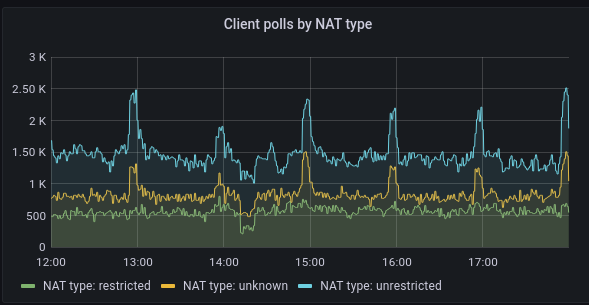
\includegraphics[width=\columnwidth]{figures/clients-by-nat}
\caption{Snowflake client poll counts by NAT type.}
\label{fig:clients-by-nat}
\todo[inline]{Replace provisional figure.}
\todo[inline]{Commit source data (e.g.\ CSV) to repository.}
\end{figure}

We use a different technique to determine the NAT type of Snowflake proxies,
because the NAT behavior discovery feature
is not exposed in the WebRTC API available to web browsers.
We adapt a technique from MassBrowser~\cite[\S \mbox{V-A}]{Nasr2020a},
and have proxies attempt to establish a connection with a peer under our control,
which is behind a simulated symmetric NAT.
If the connection is successful,
the proxy's NAT type is ``unrestricted''
and it is eligible to be matched with any client;
if not, it is ``restricted''
and may only be matched with unrestricted clients
(those without symmetric NATs).
Clients and proxies
retest their NAT type periodically, to account for changes in their local networking
environment.

We have a number of
mechanisms in place to avoid too much reliance on single points of failure.
When a proxy cannot determine its NAT type,
it goes in the ``unknown'' pool and may only be matched to unrestricted clients.
If a proxy was previously able to determine its NAT type,
a~failure of a periodic retest will not cause it to transition to the ``unknown'' type.
A~proxy that self-tests as unrestricted,
but which nevertheless fails multiple client connections in a row,
will reclassify itself as restricted
until its next successful NAT check.

The majority of browser-based Snowflake proxies
fall into the ``restricted'' NAT type.
Due to their having either port-restricted or symmetric NATs,
they are not suitable for restricted clients.
\autoref{fig:proxies-by-nats} shows the distribution of proxies by NAT type.
Despite this, we have managed to maintain a sufficient number of unrestricted proxies,
thanks in large part to the standalone, command-line
version of the Snowflake proxy.

\begin{figure}
\framebox[\columnwidth]{\vbox to 2in{\vfil\centering TODO\vfil}}
\caption{Proxy counts by NAT type.}
\label{fig:proxies-by-nats}
\end{figure}

At the same time as the snowflake proxy makes a connection to its assigned client,
% "At the same time": https://gitlab.torproject.org/tpo/anti-censorship/pluggable-transports/snowflake/40228
it also connects to the bridge.
In~contrast to the client--proxy link,
the proxy--bridge link
uses the WebSocket protocol~\cite{rfc6455}, not WebRTC.
WebSocket offers a TCP-like, point-to-point, client--server connection
layered atop HTTPS.
As we assume the danger from a censor is past
once a client reaches a snowflake proxy,
the choice of protocol for the next hop to the bridge is somewhat arbitrary.
It just needs to be a protocol that is supported in browsers
and has reasonable performance.
WebRTC would fit the bill for this link too,
but WebSocket is somewhat less complex and easier to program.

At the end of this phase,
a temporary snowflake proxy has made two connections,
one to its client and one to the bridge.
It~then proceeds to proxy a data stream between them
in both directions,
until the client terminates the session,
or the proxy itself stop operating
(when the web browser it is running in closes, for example).

\subsection{Data transfer}
\label{sec:data-transfer}

No complicated processing takes place at the proxy.
The main value if a snowflake proxy is its IP address---it
gives the client somewhere to connect to that the censor does not know about yet.
Having provided that, the proxy assumes a role
of pure data transfer until it, or one of the endpoints, goes away.
Snowflake proxies are simple conduits that transfer
a bidirectional data stream between endpoints,
without interpreting~it.
In particular, the proxy may not interfere with any
end-to-end secure information exchanged between client and bridge,
which in our deployment using Tor,
includes not only the contents of the client's streams
but also their eventual destination.
It~may be considered an instance of the
``untrusted messenger'' model described by
Feamster et~al.~\cite[\S 3]{Feamster2003a}:
what they call a ``messenger'' is our snowflake proxy;
their ``portal'' is our bridge.

The full stack of protocol layers is shown below.
We will describe each one and its purpose
in the paragraphs that follow.

\begin{verbatim}
UDP  \ WebRTC       \
DTLS | data channel | ephemeral, per proxy
SCTP /              /
KCP  \ Turbo        \
smux / Tunnel       | persistent, per session
Tor protocol        /
client streams
\end{verbatim}
\todo[inline]{Redraw ASCII art as a proper figure.}

Communication between the client and the snowflake proxy
takes place over
a WebRTC data channel~\cite{rfc8831}, which
provides a TCP-like
reliable stream interface over a UDP-based carrier.
Reliability comes from an embedded layer of
Stream Control Transmission Protocol (SCTP), which
does reordering and retransmission of dropped packets---similar
to what an OS kernel does for a TCP connection,
but in userspace.
SCTP packets are then encapsulated in Datagram TLS (DTLS)
for confidentiality and integrity between the WebRTC peers.
The peers mutually authenticate one another
at the DTLS layer using certificate fingerprints
that were exchanged during rendezvous~\cite[\S 5.1]{rfc8842}.
DTLS records are placed in UDP datagrams for transport.
The UDP--DTLS--SCTP combination comes as a packaged unit
that cannot be decomposed using the interfaces available to web browsers.

Data channels are a convenient abstraction for Snowflake,
because transmission of reliable,
connection-oriented streams data is closely matched
to the use case of a circumvention proxy.
But data channels are not the only available option:
WebRTC also provides media stream,
for unreliable transmission of real-time audio and video.
Data channels and media streams have distinguishable wire representations
that give rise to fingerprinting concerns we take up in \autoref{sec:fingerprinting}.

If snowflake proxies were as reliable as traditional proxies,
what we have described so far would already suffice:
send client traffic through the WebRTC data channel,
and have the proxy relay it to the bridge.
But Snowflake's temporary proxies might
disappear at any moment,
and the design must account for that.
If the client is in the middle of a long download,
for example, the failure of a proxy should not interrupt it:
the client and the bridge need a shared notion of session state
that is independent of any single temporary proxy connection,
so that the download can be resumed where it left off,
once connectivity is restored on a new proxy.

To make this possible, we employ the
Turbo Tunnel design pattern~\cite{Fifield2020a};
that is, we interpose an additional, userspace,
session/reliability layer between the raw transport layer
and client application streams.
This additional layer gives the proxy and the bridge
shared end-to-end state that persists throughout
the sequence of temporary proxies that are the carriers of a Snowflake session.
For the embedded session/reliability layer
we use a combination of
KCP~\cite{kcp} and
smux~\cite{smux}:
KCP provides reliability and reordering,
and smux detects the end of idle sessions and terminates them.
There is nothing essential about KCP/smux;
any other transport protocol that provides the necessary features
and can be implemented in userspace would~do,
such as QUIC, TCP, or (an additional layer of) SCTP.
(In~fact, we prototyped successfully with QUIC, before settling on KCP/smux.)
The Turbo Tunnel layer does not depend on any browser features,
because its packets are encapsulated into the data channel;
from the proxy's point of view, it's just a sequence of bytes.
A~switch from one temporary proxy to another
is invisible to the upper application layers,
except for a brief delay in packet delivery.
The failure of a proxy
is not fatal to a Snowflake session,
just as a dropped packet does not mean the end of a TCP connection.

% we tried it without Turbo Tunnel (see timeline), was not fun

Snowflake's Turbo Tunnel layer
is partially redundant with the data channel SCTP layer
on the WebRTC link between client and proxy,
which similarly builds a reliable stream interface
on an unreliable substrate.
\todo{Clarify/\allowbreak refine this in light of the fact that
\href{https://lists.torproject.org/pipermail/anti-censorship-team/2023-March/000286.html}{data channels can be unreliable and unordered}.}
The duplication is, in any case, unavoidable:
the data channel's SCTP layer is walled off by abstractions
in the WebRTC APIs available to browsers.
But more significantly, Snowflake requires an
\emph{end-to-end} notion of a session,
between the client and the bridge,
whereas the WebRTC data channel is only a
\emph{hop-by-hop} session
whose lifetime is tied to a single temporary proxy.

The combination of data channels and an inner Turbo Tunnel layer
provide a long-lasting ``virtual'' connection between the client and the bridge
that is composed of a sequence of ``real'' connections through temporary proxies.
Conceptually, here Snowflake's circumvention task is finished:
the client only needs to somehow tell the bridge, through the tunnel,
what resources to fetch, and the bridge fetches them and returns them through the tunnel.
Practically, we need to specify some concrete proxy protocol to fill this role.
This is another place where anything reasonable will serve,
with the caveat that it should be an encrypted protocol
(secure between client and bridge) to prevent proxies
from inspecting or interfering with the client's requests.
(The client--proxy link is encrypted with DTLS
and the proxy--bridge link with HTTPS,
but in the middle of these the proxy is in a position to see
the client's traffic, unless separately end-to-end encrypted.)
Our deployment is built on Tor,
and the bridge in our deployment is a Tor entry relay.
The Tor client provides a local SOCKS interface,
which fills the role of an encrypted proxy protocol,
and users of course get Tor's anonymity and privacy benefits
in addition to the blocking resistance supplied by Snowflake.
(In our deployment, not even the bridge is fully trusted---it
does not get to see the contents of clients' connection,
nor their eventual destinations.)
But there is nothing about Tor that Snowflake depends on essentially;
the tasks of providing a blocking-resistant to the bridge
and then telling the bridge what to do are easily separable.
We discuss alternatives to Tor
and other extensions of Snowflake in \autoref{sec:future}.
Integration with Tor brings its own challenges,
which we will get into in \autoref{sec:challenges}\todo{Check this cross reference when \autoref{sec:experience} is fleshed out.}.

\section{Protocol fingerprinting}
\label{sec:fingerprinting}

% https://gitlab.torproject.org/tpo/anti-censorship/pluggable-transports/snowflake/-/wikis/Fingerprinting

Snowflake leans heavily into the ``address blocking'' side of blocking resistance,
but the ``content blocking'' part matters too.
As always, the goal is to make circumvention traffic
difficult to distinguish from traffic the censor cares not to block.
Snowflake is, by nature, tied to WebRTC,
and therefore can only be effective against a censor
that is not motivated to block WebRTC protocols wholesale.
But even within that scope,
there are many possible variations in \emph{how}
WebRTC is implemented and used,
which, if not considered carefully, might permit a censor
to selectively block only Snowflake,
while leaving other uses of WebRTC undisturbed.
In~this discussion, it is worth remembering
what Tschantz et~al.\ have observed\cite[\mbox{VI-A}]{Tschantz2016a}:
that censors prefer to exploit
simple, precise, deterministic distinguishers
that appear in the early phase of a circumvention session whenever possible,
and use long-term, probabilistic, or computationally expensive tests
only as a last resort.
It is hardly worth worrying about protocol fingerprints
in a circumvention system while easier distinguishers exist;
conversely, small, patchable, fingerprinting flaws are forgivable
as long as the foundation is solid.

As~WebRTC is designed for the web,
most implementation of WebRTC are embedded in web browsers,
and are not trivially usable outside that context.
Snowflake originally used a WebRTC library extracted from Chromium,
but that eventually proved unworkable from a practical standpoint---more
details are in \autoref{sec:deployment}.
Since 2019, Snowflake has used Pion~\cite{pion-webrtc},
% "Evaluate pion WebRTC" https://bugs.torproject.org/tpo/anti-censorship/pluggable-transports/snowflake/28942
an independent implementation of WebRTC
implemented as a generic library,
not tied to any browser.
This is both good and bad.
The good is greater agility and less development friction,
and a working relationship with upstream developers
that enables us to get fingerprinting-related changes made.
The bad is that the WebRTC fingerprint of Pion
does not automatically match that of the primarily browser-originated
WebRTC that Snowflake aims to blend in with.

Unfortunately for the circumvention developer,
the rich set of interacting protocols that comprise WebRTC
afford a large attack surface for fingerprinting.
Not only that, WebRTC leaves the details of
the signaling path---where peers exchange information
needed to set up a connection,
corresponding to Snowflake rendezvous---unspecified~\cite[\S 3]{rfc8825},
leaving applications to invent their own signaling mechanisms.
% "The choice of protocols for client-server and inter-server signaling, and the definition of the translation between them, are outside the scope of the WebRTC protocol suite described in this document."
% https://www.rfc-editor.org/rfc/rfc8829.html#section-3.1: "JSEP does not specify a particular signaling model or state machine, other than the generic need to exchange session descriptions in the fashion described by [RFC3264] (offer/answer)..."

The following is a list of potential fingerprinting concerns
that bear on Snowflake, together with brief descriptions
of the degree to which we have tried to address them.
The list may not be exhaustive.

\begin{description}
\item[Selection of STUN servers]
It~is not unusual for a WebRTC application to use STUN;
but which servers it uses is externally observable
and is the choice of the application (often hardcoded).
Running a dedicated STUN server just for Snowflake is a nonstarter---if~there
are no users of the server other than circumvention users,
a~censor will experience no harm in simply blocking its IP address.
In~Snowflake, we use a pool of public STUN servers,
used for many purposes other than circumvention,
and filtered for those that support the NAT behavior discovery feature
described in \autoref{sec:ice}.
The client chooses a random subset of the servers in the pool
each time it makes a connection.
This is because not every STUN server is accessible
under every censor.
% I went to check stun.l.google.com for blocking in China,
% but OONI apparently does not measure that server:
% https://explorer.ooni.org/chart/mat?test_name=stunreachability&axis_x=measurement_start_day&since=2023-02-12&until=2023-03-15&time_grain=day&probe_cc=CN&axis_y=domain

\item[Format and content of STUN messages]
STUN messages consist of a fixed header
followed by a variable-length list of ordered
attributes~\cite[\S 5]{rfc8489}.
STUN is most often deployed using plaintext UDP as a transport,
which leaves its messages open to inspection
and potentially fingerprintable.
What attributes appear,
and their relative order,
is a property of the the implementation
and the way the application uses STUN.
Among the attributes are some used
for the NAT behavior discovery feature~\cite[\S 7]{rfc5780}
of \autoref{sec:ice}.

\todo{Have we done anything for STUN message fingerprinting?}

\item[Rendezvous]
The rendezvous methods of
\autoref{sec:rendezvous},
being modular,
generally all need their own security argument
as to why they should be difficult to block.
Besides that, each must be implemented in a way
that does not expose accidental distinguishers.
For example, the domain fronting and AMP cache rendezvous methods
use HTTPS, which is TLS, which means they are susceptible to TLS fingerprinting~\cite[\S 5.1]{Fifield2015a}.
In Snowflake, we use the uTLS package~\cite[\S VII]{Frolov2019a}
(commonly used by circumvention programs)
to get a TLS fingerprint that is randomized or that imitates common browsers.
See \autoref{sec:block-ir} for an account of when
domain fronting rendezvous was briefly blocking in Iran,
because we were slow in activating uTLS.

Though each rendezvous method must be difficult to block in itself,
a~censor may combine a low-confidence suspicion of having observed a rendezvous exchange
with features from other phases of the Snowflake data exchange
to strengthen its guess and possibly effect a blocking decision.

\item[DTLS]
DTLS over UDP is the outermost protocol
of a WebRTC data connection and is exposed to the censor.
DTLS is an adaptation of TLS to the datagram setting,
and therefore inherits the fingerprinting concerns of TLS~\cite{Frolov2019a}.
TLS/DTLS fingerprinting may involve, for example,
inspecting the ClientHello message to see what
ciphersuites and extensions are used,
and their ordering---it may be that a particular fingerprint
is specific to a particular implementation of a circumvention system
and may therefore be blocked at low cost to the censor.

Due to practical implementation considerations,
the defenses to DTLS fingerprinting in Snowflake are not very robust,
and are reactive rather than proactive.
In~the world of TLS one may use the uTLS package~\cite[\S VII]{Frolov2019a},
or~(at a not inconsiderable cost of complexity)
tunnel through a locally installed web browser
to borrow its TLS fingerprint~\cite[\S 5.1]{Fifield2015a}.
But there is as yet no equivalent of uTLS for DTLS,
and using a browser's DTLS implementation proved unworkable
even for implementation, let alone convenient deployment to users.
The present way of altering DTLS fingerprints in Snowflake
is by submitting pull requests to the Pion project
whenever a fingerprint feature actually used for blocking is identified.
\autoref{sec:block-ru} documents how this has happened twice,
in response to blocking in Russia.

% For reference, fingerprinting changes upstreamed to Pion:
% * IP addresses as SNI values
%   https://bugs.torproject.org/tpo/anti-censorship/pluggable-transports/snowflake/40014#note_2764715
%   https://github.com/pion/dtls/issues/406
%   https://github.com/pion/dtls/pull/407
% * supported_groups in Server Hello
%   https://bugs.torproject.org/tpo/anti-censorship/pluggable-transports/snowflake/40014#note_2765074
%   https://github.com/pion/dtls/issues/409
%   https://github.com/pion/dtls/pull/410
% * Server sending Hello Verify Request
%   https://bugs.torproject.org/tpo/anti-censorship/pluggable-transports/snowflake/40014#note_2764715
%   https://gitlab.torproject.org/tpo/applications/tor-browser-build/-/merge_requests/637
%   https://bugs.torproject.org/tpo/anti-censorship/pluggable-transports/snowflake/40249
%   https://github.com/pion/dtls/pull/513
%   https://github.com/pion/webrtc/pull/2407
%
% Not fingerprinting but also upstreamed:
% * NAT behavior detection
%   https://github.com/pion/stun/issues/8
%   https://github.com/pion/stun/pull/33

\item[Data channel or media stream]
Besides data channels, WebRTC offers \firstterm{media streams},
in line with its intended purpose of enabling real-time
audio and video communication.
Data channels and media streams are externally distinguishable
because they use different encrypted transports:
while data channels use DTLS,
media streams use DTLS-SRTP;
that is, the Secure Real-Time Transport Protocol
preceded by a DTLS key exchange~\cite[\S 4.3]{rfc8827}.

Data channels are a better match for Snowflake's communication model:
media streams are meant to contain encoded audio and video,
not arbitrary binary data,
and do not guarantee reliable or in-order delivery.
But the use of DTLS rather than DTLS-SRTP could become
a significant feature if most other WebRTC applications use media streams.
(We do not know which is more common in practice,
or whether there are enough other uses of data channels
to support an argument that blocking all data channels would be expensive.)
Although it would be less convenient,
it would be possible to adapt the WebRTC link between
the client and the proxy
to use a media stream rather than a data channel,
either by modulating binary data into a well-formed encoded
audio or video signal in the manner of, say,
CovertCast~\cite[\S 4.3]{McPherson2016a},
or by directly replacing the ciphertext of SRTP packets,
like Protozoa~\cite[\S 4.4]{Barradas2020a}.
% See idea about WebRTC Encoded Transform: https://lists.torproject.org/pipermail/anti-censorship-team/2023-February/000284.html

\end{description}

The degree of Snowflake's susceptibility to protocol fingerprinting
has been analyzed in the past by
Fifield and Gil Epner~\cite{arxiv.1605.08805} and by
MacMillan et~al.~\cite{arxiv.2008.03254}.
The former predates Snowflake's switch to Pion,
which changed its protocol fingerprints at multiple layers.
The latter identified specific distinguishing features
of the Pion DTLS handshake
that later ended up being used in practice
to block Snowflake in Russia
and which we had to work around;
see \autoref{sec:block-ru}.

Chen et~al.~\cite{Chen2023a}
have the good idea of combining features
of rendezvous and the DTLS handshake
to reduce false positives.
They first prefilter using DNS queries:
the Snowflake client's default selection of STUN servers
on its own may be unexceptional,
and its default server used for domain fronting rendezvous
on its own may be unexceptional,
but DNS queries for all of these within a short time span
is likely characteristic of Snowflake and little else.
After DNS prefiltering, they identify Snowflake connections
by DTLS fingerprinting of the Pion implementation of DTLS
used in the Snowflake client.
The authors acknowledge that DTLS fingerprinting
is fragile, as the DTLS fingerprint is, in principle,
a~controllable feature.
The DNS query prefilter may perhaps be mitigated
by alternative rendezvous methods (\autoref{sec:rendezvous}),
or by smarter selection of STUN servers by the client.

Somewhat related to protocol fingerprinting is traffic analysis;
that is, inferring the use of a censorship system
by looking at features like the distribution of packet sizes,
arrival times, and the sequence of packet directionality (in/out)---the
kind of analysis that, in other contexts, is known as ``website fingerprinting''
% Could cite IETF survey on website fingerprinting.
% (But don't want to give this topic more attention than it is due.)
may potentially also be applied to detecting circumvention systems.
In~our opinion, this possibility has remained more potential than actual.
As our own (see \autoref{sec:experience}) and wider experience shows,
censors still prefer to attack easier targets.
The Snowflake protocol supports traffic shaping (inside the WebRTC layer),
but it is currently disabled:
packets are sent with their ``natural'' sizes and without delay,
reflecting the traffic dynamics of the tunneled Tor traffic
(which in turn more or less represents the dynamics
of the user's application-layer streams deeper in the tunnel).
Circumvention research awaits a treatment of
what is a good strategy for traffic shaping to
best mitigate attacks of this nature,
and an analysis of how much of a threat they pose in practice.

\section{Experience}
\label{sec:experience}

\subsection{Deployment history}
\label{sec:deployment}

% Excerpts from https://gitlab.torproject.org/tpo/network-health/metrics/timeline:
% |2017-01-24|||snowflake|Tor Browser 7.0a1 released, including Snowflake for GNU/Linux only.|[blog post](https://blog.torproject.org/blog/tor-browser-70a1-released)||
% |2017-08-08|||snowflake|Tor Browser 7.5a4 released, including Snowflake for macOS.|[blog post](https://blog.torproject.org/blog/tor-browser-75a4-released) [issue](https://bugs.torproject.org/tpo/applications/tor-browser/22831)||
% |2018-03-26 20:43:42|||snowflake|Release of Tor Browser 8.0a5. Improves snowflake client performance.|[blog post](https://blog.torproject.org/tor-browser-80a5-released) [ticket](https://bugs.torproject.org/tpo/anti-censorship/pluggable-transports/snowflake/21312)||
% |2019-10-01|||snowflake|Release of Tor Browser 9.0a7, the first release that has Snowflake for Windows.|[blog post](https://blog.torproject.org/new-release-tor-browser-90a7) [ticket](https://bugs.torproject.org/tpo/anti-censorship/pluggable-transports/snowflake/25483)||
% |2020-05-22 19:51:29|||snowflake|Release of Tor Browser 9.5a13, the first release with Turbo Tunnel session persistence features for Snowflake. There is a spike in estimated users on 2020-05-21 and 2020-05-22, which appears to be an artifact.|[blog post](https://blog.torproject.org/new-release-tor-browser-95a13) [ticket](https://bugs.torproject.org/tpo/applications/tor-browser/34043) [users graph](https://metrics.torproject.org/userstats-bridge-transport.html?start=2020-03-01&end=2020-08-01&transport=snowflake)||
% |2020-06-02 18:09:48|||snowflake|Release of Tor Browser 10.0a1, the first release with Snowflake for Android.|[blog post](https://blog.torproject.org/new-release-tor-browser-100a1) [ticket](https://bugs.torproject.org/tpo/applications/tor-browser/30318)||
% |2020-06-25|2020-06-25||snowflake|One- or two-day spike in estimated Snowflake users. It resembles the spike that occurred around the time of the Turbo Tunnel release of Tor Browser 9.5a13 on 2020-05-22.|[users graph](https://metrics.torproject.org/userstats-bridge-transport.html?start=2020-03-01&end=2020-08-01&transport=snowflake)|X|
% |2021-07-06 16:56:37|||snowflake|Release of Tor Browser 10.5, first stable release that includes Snowflake.|[blog post](https://blog.torproject.org/new-release-tor-browser-105)||
% |2021-12-20|||snowflake|Release of Tor Browser 11.0.3, with an altered DTLS fingerprint in Snowflake to counteract blocking in Russia.|[blog post](https://blog.torproject.org/new-release-tor-browser-1103/) [issue](https://bugs.torproject.org/tpo/applications/tor-browser-build/40393) [NTC post](https://ntc.party/t/ooni-reports-of-tor-blocking-in-certain-isps-since-2021-12-01/1477/59)||
% |2021-12-14|||snowflake|Release of Tor Browser 11.5a1, with an altered DTLS fingerprint in Snowflake to counteract blocking in Russia.|[blog post](https://blog.torproject.org/new-release-tor-browser-115a1/) [issue](https://bugs.torproject.org/tpo/applications/tor-browser-build/40393) [NTC post](https://ntc.party/t/ooni-reports-of-tor-blocking-in-certain-isps-since-2021-12-01/1477/59)||
% |2022-01-25 17:41:00|||snowflake|Switched the snowflake bridge to a temporary load-balanced staging server. Debugged connection problems until 2022-01-25 18:47:00.|[issue](https://bugs.torproject.org/tpo/tpa/team/40598#note_2772287) [comment](https://bugs.torproject.org/tpo/anti-censorship/pluggable-transports/snowflake/40095#note_2772325) [post](https://forum.torproject.net/t/tor-relays-how-to-reduce-tor-cpu-load-on-a-single-bridge/1483/16) [comment](https://github.com/net4people/bbs/issues/103#issuecomment-1033067920)||
% |2022-03-16 16:51:35|||snowflake|Moved Snowflake traffic to the interim bridge running instances flakey1–flakey8.|[comment](https://bugs.torproject.org/tpo/tpa/team/40664#note_2787624)||
% |2022-07-14|||bridge|Release of Tor Browser 11.5, with a new feature of automatic censorship circumvention configuration.|[blog post](https://blog.torproject.org/new-release-tor-browser-115/)||

The deployment of Snowflake to end users was gradual,
reflecting its development.
It was tested in the alpha release series of Tor Browser
over a course of four years
before finally becoming part of the stable release.
% https://gitlab.torproject.org/tpo/anti-censorship/pluggable-transports/snowflake/-/issues/19001 "First working bundles with Snowflake, for linux only"
The necessary go-webrtc bindings became available first for GNU/Linux,
and so Snowflake was released for the first time, for GNU/Linux only,
with Tor Browser 7.0a1 on \mbox{2017-01-24}.
% https://gitlab.torproject.org/tpo/anti-censorship/pluggable-transports/snowflake/-/issues/19001 "mac reproducible build"
% [tbb-dev] Please check reproducibility of mac build with Snowflake (e084e83418) https://lists.torproject.org/pipermail/tbb-dev/2017-July/000579.html
The next platform for which we got go-webrtc bindings working
and building reproducibly was macOS,
and Snowflake for macOS was released as part of
Tor Browser 7.5a4 on \mbox{2017-08-08}.

% https://gitlab.torproject.org/tpo/anti-censorship/pluggable-transports/snowflake/-/issues/19001 "windows reproducible build"
% https://gitlab.torproject.org/tpo/anti-censorship/pluggable-transports/snowflake/-/issues/25483 "Windows reproducible build of snowflake"
Preparing reproducible the go-webrtc bindings for Windows
presented enormous difficulties.
The Chromium browser\todo{Maybe \mbox{``libwebrtc''} is better than ``Chromium''.}
from which go-webrtc was derived
is a massively complex software project,
with a multi-stage and frequently changing build system.
The reproducible build environment,
with its requirements to
cross-compile from source,
without any pre-built binary or proprietary dependencies,
was never a supported build configuration.
The issue stalled us for a long time.
We finally broke through the impasse
by switching from the Chromium-derived go-webrtc
to Pion WebRTC~\cite{pion-webrtc} in the middle of 2019.
% https://gitlab.torproject.org/tpo/anti-censorship/pluggable-transports/snowflake/-/issues/28942 "Evaluate pion WebRTC"
Pion is an independent implementation of WebRTC protocols, written in Go,
that had not existing at the beginning of the Snowflake project.
Pion presented no major difficulties to building reproducibly,
and with it we were able to release Snowflake for Windows
in Tor Browser 9.0a7 on \mbox{2019-10-01}.

While at this point Snowflake was functional on all major desktop platforms,
it was not yet really usable.
The reason is that there was no session persistence:
a~user's Tor browsing session was tied to the first Snowflake proxy they were assigned by the broker.
If the user was lucky, the proxy might persist for an hour;
if unlucky, only a few minutes;
and then the user would have to restart their browser---there was
no way to start using a different proxy on the fly.
(A~lack of session persistence across temporary proxies
had also been a problem in flash proxy~\cite[\S 5.2]{Fifield2012a}.)
Probably because of this, by early 2020,
the number of simultaneous users of Snowflake
had not risen above~40.
% > library("tidyverse")
% > WANTED_FINGERPRINTS <- c(
%     "5481936581E23D2D178105D44DB6915AB06BFB7F" = "snowflake-01",
%     "91DA221A149007D0FD9E5515F5786C3DD07E4BB0" = "snowflake-02"
%   )
% > userstats <- read_csv("figures/users-global/userstats-bridge-transport-multi.csv") %>%
%     filter(transport == "snowflake" & fingerprint %in% names(WANTED_FINGERPRINTS)) %>%
%     mutate(users = users * frac / 100, frac = NULL) %>%
%     group_by(date, transport) %>% summarize(users = sum(users, na.rm = TRUE), .groups = "drop")
%
% Ignoring two apparently anomalous spikes before 2021.
% One on 2020-05-21 and 2020-05-22 (the day of the Turbo Tunnel release):
% > filter(userstats, "2020-05-19" <= date & date <= "2020-05-24")
% # A tibble: 6 x 3
%   date       transport  users
%   <date>     <chr>      <dbl>
% 1 2020-05-19 snowflake   9.16
% 2 2020-05-20 snowflake  13.6
% 3 2020-05-21 snowflake 134.
% 4 2020-05-22 snowflake 388.
% 5 2020-05-23 snowflake   7.9
% 6 2020-05-24 snowflake  13.9
% One on 2020-06-25 and 2020-06-26 (not sure what this one is about):
% > filter(userstats, "2020-06-23" <= date & date <= "2020-06-28")
% # A tibble: 6 x 3
%   date       transport users
%   <date>     <chr>     <dbl>
% 1 2020-06-23 snowflake  17.0
% 2 2020-06-24 snowflake  20.2
% 3 2020-06-25 snowflake  71.7
% 4 2020-06-26 snowflake 211.
% 5 2020-06-27 snowflake  22.5
% 6 2020-06-28 snowflake  33.7
%
% > filtered <- filter(userstats, !(date %in% as.Date(c("2020-05-21", "2020-05-22", "2020-06-25", "2020-06-26"))))
% > filtered[which.max(filter(filtered, date < "2020-05-21")$users), ]
% # A tibble: 1 x 3
%   date       transport users
%   <date>     <chr>     <dbl>
% 1 2020-04-01 snowflake  34.0
The Turbo Tunnel session persistence feature
described in \autoref{sec:data-transfer}
became available to users in Tor Browser 9.5a13
on \mbox{2020-05-22}.
% https://gitlab.torproject.org/tpo/anti-censorship/pluggable-transports/snowflake/-/issues/33745 "Merge a turbotunnel branch"
% https://gitlab.torproject.org/tpo/applications/tor-browser/-/issues/34043 "Update snowflake to persist sessions across proxies"
It was at this point that Snowflake became
comfortable enough to use for daily browsing,
and the number of users began to grow steadily into 2021.\todo{Add NAT matching to this timeline: that was required for comfort as well.}
Snowflake for Android became available with
Tor Browser 10.0a1 on \mbox{2020-06-02}.
% https://gitlab.torproject.org/tpo/applications/tor-browser/-/issues/28672 "Android reproducible build of Snowflake"

\begin{figure*}
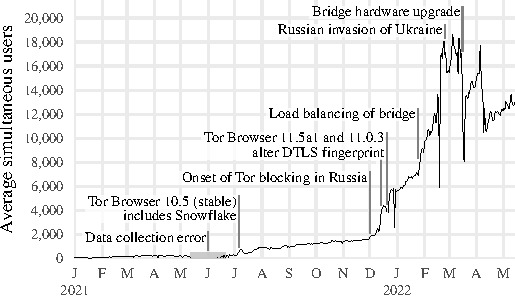
\includegraphics{figures/users-global/users-global}
\caption{
Estimated average number of simultaneous Snowflake users per day.
The value at the extreme left edge of the graph,
the beginning of 2021, is about~60.
At this point, Snowflake was available in the Tor Browser alpha release series
for desktop platforms and Android,
and it had the Turbo Tunnel session persistence feature.
% Loesing~\cite{tor-tr-2012-10-001} describes how user counts are estimated.
The maximum value in the part of the graph not shown
is 133, on \mbox{2020-12-09}.
% > filtered[which.max(filter(filtered, date < "2021-01-01")$users), ]
% # A tibble: 1 x 3
%   date       transport users
%   <date>     <chr>     <dbl>
% 1 2020-12-09 snowflake  133.
}
\label{fig:user-counts}
\todo[inline]{Cut off the \(y\)-axis at the maximum of the data,
so that the vertical annotations at the top fall outside the plot itself.}
\todo[inline]{Bandwidth chart? Ideally with aligned horizontal axis.}
\end{figure*}

This brings us to \autoref{fig:user-counts},
which shows the estimated number of Snowflake users since 2021.
Because of Snowflake's affiliation with Tor and Tor Browser,
we estimate users using the normal statistics reported by the bridge
and collected by Tor Metrics.
Be aware: the chart does not show the number of unique daily users,
as one might expect,
but the \emph{average number of simultaneous users} per day.
For example, if the line goes through 1,700 on 2021-12-01,
it means that if the number of Snowflake users were instantaneously sampled
at a random moment in that day, the expected number of users would be 1,700.
The number of unique users per day is necessarily higher,
but how much higher depends on how many hours an average user stays connected.
Counting simultaneous users, rather than unique users,
has been the practice of Tor Metrics since 2012~\cite{tor-tr-2012-10-001};
the reason for it is that the statistics reported by Tor bridges
lend themselves better to the former estimation than the latter.
\todo{Can we do better with respect to unique users? See \href{https://bugs.torproject.org/tpo/network-health/metrics/analysis/40012\#note_2803514}{\#40012}.}
The values should not be taken as exact---the
algorithm involves some approximations and guessed parameters---but
the chart is at least relatively comparable to others
produced by Tor Metrics.\todo{%
Speaking of, should we show Snowflake numbers in context with other PTs and relay users?
% https://gitlab.torproject.org/tpo/community/support/-/issues/40050#note_2796770 "This graph shows shows all the Tor users in Russia, whether using relays, bridges, or bridges with pluggable transports."
}

The growth of Snowflake users began in earnest on
\mbox{2021-07-06}, when it became part of the stable release series
in Tor Browser~10.5.
% https://blog.torproject.org/new-release-tor-browser-105
Being part of the stable series means that it was
available as a built-in option for circumvention for all Tor Browser users,
not only those who had taken the trouble to install a special alpha release.
The rate of adoption increased,
and the number of simultaneous users steadily increased to almost 2,000
over the next five months.

On \mbox{2021-12-01}, some (not all) ISPs in Russia began to block
most forms of access to Tor~\cite{ooni-2021-russia-blocks-tor}\todo{Possibly replace with ``Network Responses to Russia's Invasion of Ukraine'' (\S6.2), to appear USENIX 2023.}.
We will have more to say about this in \autoref{sec:block-ru}.
Snowflake was also affected,
but we released updates to evade the blocking on
\mbox{2021-12-14} (alpha) and
\mbox{2021-12-20} (stable).
The blocking of plain Tor increased demand for circumvention transports,
and Snowflake was strongly affected.
The number of users quadrupled in the next two months.
There were so many new users from Russia, in fact,
that we had to rearchitect the bridge deployment
at the end of January
in order to handle the increased load.
% https://forum.torproject.net/t/tor-relays-how-to-reduce-tor-cpu-load-on-a-single-bridge/1483
% https://bugs.torproject.org/tpo/anti-censorship/pluggable-transports/snowflake/40095#note_2772325
Even with these architectural changes,
the bridge's CPU capacity again became saturated.
Around the beginning of March, Snowflake was almost unusably slow for a few weeks.
% https://old.reddit.com/r/TOR/comments/t49i14/hello_i_have_a_problem_with_snowflake_can_you/
% https://forum.torproject.net/t/tor-project-more-resources-required-for-snowflake-bridge/2353
The invasion of Ukraine by Russia starting on \mbox{2022-03-24}
was accompanied by additional restrictions on Internet access in Russia,
which only increased demand for circumvention.
In response, on \mbox{2022-03-16} we upgraded the bridge to substantial server hardware,
which has been sufficient for the time being.
(See \autoref{sec:future} for an idea to run multiple independent bridge sites,
to permit scaling further.)
As of May 2022, about 65\% of Snowflake users come from Russia.
% https://metrics.torproject.org/collector.html#type-bridge-extra-info
%
% @type bridge-extra-info 1.3
% extra-info flakey3 5481936581E23D2D178105D44DB6915AB06BFB7F
% published 2022-05-20 21:10:47
% transport snowflake
% dirreq-v3-ips ru=12216,us=1640,cn=704,de=400,gb=296,by=272,in=224,??=208,ua=168,fr=160,ir=136,nl=128,ca=88,br=80,it=80,au=72,pl=72,sa=72,es=64,se=64,ch=48,cz=48,mx=48,tr=48,ae=40,jp=40,ro=40,za=40,at=32,eg=32,id=32,co=24,dk=24,dz=24,fi=24,hk=24,hu=24,no=24,ph=24,pk=24,ar=16,bd=16,be=16,cl=16,gr=16,ie=16,il=16,kr=16,kz=16,lt=16,ma=16,mm=16,my=16,ng=16,nz=16,pt=16,sg=16,sk=16,vn=16,al=8,ao=8,az=8,ba=8,bf=8,bg=8,bh=8,bj=8,bo=8,ci=8,cm=8,cr=8,cu=8,cy=8,do=8,ec=8,ee=8,et=8,eu=8,ge=8,gf=8,gh=8,gt=8,hr=8,iq=8,jm=8,jo=8,ke=8,kg=8,km=8,kw=8,lb=8,lk=8,lu=8,lv=8,ly=8,md=8,mk=8,ml=8,mo=8,mu=8,mv=8,mw=8,mz=8,na=8,om=8,pa=8,pe=8,pg=8,pr=8,py=8,qa=8,re=8,rs=8,rw=8,sb=8,sc=8,sd=8,si=8,so=8,sv=8,sy=8,th=8,tm=8,tn=8,tw=8,tz=8,ug=8,uy=8,uz=8,ve=8,ye=8,zm=8
% dirreq-v3-reqs ru=21688,us=2728,cn=1280,de=664,??=648,gb=504,by=464,fr=368,ua=344,in=336,nl=280,ir=248,ca=168,au=152,br=128,it=120,pl=112,es=96,mx=96,ro=96,sa=96,se=88,id=80,ch=72,tr=72,za=72,cz=64,jp=64,ae=56,eg=56,co=48,hk=48,at=40,dk=40,no=40,ar=32,be=32,dz=32,fi=32,ie=32,lv=32,ng=32,nz=32,ph=32,pk=32,pt=32,bd=24,hu=24,il=24,jo=24,kr=24,kz=24,vn=24,az=16,ba=16,cl=16,ec=16,et=16,ge=16,gr=16,hr=16,ke=16,lt=16,ma=16,mm=16,mu=16,my=16,pa=16,sg=16,sk=16,th=16,tm=16,tw=16,uy=16,uz=16,al=8,ao=8,bf=8,bg=8,bh=8,bj=8,bo=8,ci=8,cm=8,cr=8,cu=8,cy=8,do=8,ee=8,eu=8,gf=8,gh=8,gt=8,iq=8,jm=8,kg=8,km=8,kw=8,lb=8,lk=8,lu=8,ly=8,md=8,mk=8,ml=8,mo=8,mv=8,mw=8,mz=8,na=8,om=8,pe=8,pg=8,pr=8,py=8,qa=8,re=8,rs=8,rw=8,sb=8,sc=8,sd=8,si=8,so=8,sv=8,sy=8,tn=8,tz=8,ug=8,ve=8,ye=8,zm=8
% dirreq-v3-resp ok=32240,not-enough-sigs=0,unavailable=0,not-found=0,not-modified=3208,busy=0
% dirreq-v3-direct-dl complete=0,timeout=0,running=0
% dirreq-v3-tunneled-dl complete=27256,timeout=4948,running=32,min=963,d1=112650,d2=280773,q1=417567,d3=637384,d4=13253000,md=22649666,d6=25108500,d7=28307500,q3=31003000,d8=36534666,d9=50908500,max=121278000
% bridge-ips ru=16720,us=2744,cn=1024,de=672,gb=440,by=400,in=400,??=272,fr=264,ua=232,ir=200,nl=200,br=152,ca=152,au=136,it=136,pl=128,sa=112,se=96,tr=96,es=80,jp=80,mx=72,ro=72,ch=64,eg=64,za=64,ae=56,cz=56,at=48,id=48,co=40,dz=40,hk=40,no=40,pk=40,bd=32,be=32,fi=32,kr=32,kz=32,ng=32,pt=32,ar=24,cl=24,dk=24,gr=24,hu=24,ie=24,il=24,ma=24,my=24,ph=24,sk=24,vn=24,bg=16,cu=16,ec=16,gh=16,jo=16,ke=16,kw=16,lk=16,lt=16,lv=16,mm=16,mu=16,nz=16,sg=16,th=16,tw=16,uz=16,ye=16,al=8,ao=8,ap=8,az=8,ba=8,bf=8,bh=8,bj=8,bn=8,bo=8,ci=8,cm=8,cr=8,cy=8,do=8,ee=8,et=8,eu=8,ge=8,gf=8,gn=8,gt=8,hn=8,hr=8,iq=8,is=8,jm=8,kg=8,km=8,lb=8,lu=8,ly=8,md=8,mk=8,ml=8,mo=8,mv=8,mw=8,mz=8,na=8,np=8,om=8,pa=8,pe=8,pg=8,pr=8,ps=8,py=8,qa=8,re=8,rs=8,rw=8,sb=8,sc=8,sd=8,si=8,sn=8,so=8,sr=8,sv=8,sy=8,tm=8,tn=8,tt=8,tz=8,ug=8,uy=8,ve=8,zm=8
% bridge-ip-versions v4=23424,v6=2840
% bridge-ip-transports <OR>=8,snowflake=26264
%
% >>> 21688 / 32240 # dirreq-v3-reqs=ru / dirreq-v3-resp=ok
% 0.6727047146401985
% >>> 16720 / 26264 # bridge-ips=ru / bridge-ip-transports=snowflake
% 0.7137978142076503

\todo{2022-07-14 Tor Browser 11.5 \href{https://blog.torproject.org/new-release-tor-browser-115/}{automatic circumvention configuration}.}

The Tor Metrics Timeline~\cite{tor-metrics-timeline}
has a detailed list of events over the course of Snowflake deployment.

% david
$X$ TB of user data transferred\todo{Compute this, make it reproducible.}

\subsection{Proxy recruitment and growth}
\label{sec:proxies}

\begin{figure}
\framebox[\linewidth]{\vbox to 1.5in{\vfil\centering TODO\vfil}}
\caption{Number of Snowflake proxies over time.}
\label{fig:total-proxy-counts}
\bigskip
\framebox[\linewidth]{\vbox to 1.5in{\vfil\centering TODO\vfil}}
\caption{Snowflake proxy types over time.}
\label{fig:proxy-type-counts}
\end{figure}

The deployment of Snowflake proxies began with a bare minimum deployment
of three standalone Go proxies all on the same IP address as the Snowflake bridge,
as well as a few proxies from deployed Snowflake badges.
We began to collect metrics on the number of deployed proxies on \mbox{2019-06-29}.
\autoref{fig:total-proxy-counts} shows the total count of unique proxy IP addresses
from the beginning of our collection to the writing of this paper.
The majority of the growth in Snowflake proxies over the last three years comes from
the success of the Snowflake browser add-on.
The add-on was released for Firefox on \mbox{2019-06-26} and Chrome on \mbox{2019-07-03},
but the first major spike in proxy counts was thanks to the integration
of Snowflake with the existing flash proxy add-on, Cupcake.
The number of Cupcake proxies dropped off completely later that year,
but Snowflake add-on usage had already risen to compensate.
Currently, the vast majority of Snowflake proxies are from the browser add-on,
as shown in \autoref{fig:proxy-type-counts}.

While early growth in the number of unique Snowflake proxy IPs
was due to the development of easier deployment methods and UX features for proxy volunteers,
the later growth in proxy counts was due to outreach
and follows the increase in demand for Snowflake proxy capacity from the increase in client usage. 

Counts of web badge vs. browser add-on vs. standalone daemon
Timeline of proxy + webext deployment
% |2019-06-26|||snowflake|Deployed version 0.0.1 of the Snowflake WebExtension for Firefox.|[comment](https://bugs.torproject.org/tpo/anti-censorship/pluggable-transports/snowflake/30931#note_2593598)||
% |2019-07-03|||snowflake|Deployed version 0.0.1 of the Snowflake WebExtension for Chrome.|[comment](https://bugs.torproject.org/tpo/anti-censorship/pluggable-transports/snowflake/30999#note_2593718)||
Cupcake
Relative ineffectiveness of web badge (i.e. the flash proxy model)
people love the add-on and the daily count of connections
We decided early on that the opt-out proxying model had been a mistake,
and that Snowflake would be only opt-in.

Orbot? as both client and proxy?

\subsection{Development challenges}
\label{sec:challenges}

% arlo, cecylia

Difficulty of using WebRTC outside a browser

Reproducible builds
- difficulty of cross-compiling go-webrtc extracted from Chromium

History of changing domain fronts

scaling
% david
- load balancing
- multi-bridge

The Snowflake system
admittedly contains a lot of moving parts.
Some complexity is inherent in the nature
of what we are building:
Snowflake is more complicated than a static encrypted proxy
and always will be.
Complexity is the enemy of security and robustness, however,
and in a system meant for real production use
could even be considered an existential risk,
if the demands of maintenance exceed what the maintainers can provide.
Managing complexity and designing for low maintenance
are material concerns,
and must sometimes take priority over speed of development.

% Safe Browsing / zip bomb problem (2019)
% https://gitlab.torproject.org/tpo/anti-censorship/pluggable-transports/snowflake/-/issues/31250


\subsection{Blocking in Turkmenistan}
\label{sec:block-tm}

\begin{figure}
\framebox[\linewidth]{\vbox to 2in{\vfil\centering TODO\vfil}}
\caption{
Users in Turkmenistan and Russia,
around blocking events.
}
\label{fig:user-counts-tm-ru}
\end{figure}

% |2021-10-24||tm|snowflake|Snowflake users in Turkmenistan drop to zero, possibly as a result of blocking of the broker's domain-fronting channel.|[issue](https://bugs.torproject.org/tpo/anti-censorship/censorship-analysis/40024) [comment](https://bugs.torproject.org/tpo/community/support/40030#note_2759213) [discussion](http://meetbot.debian.net/tor-meeting/2021/tor-meeting.2021-11-04-15.59.log.html#l-55)|X|

\url{https://bugs.torproject.org/tpo/anti-censorship/censorship-analysis/40024}

\autoref{fig:user-counts-tm-ru}

Block of domain front
Unclear if AMP cache rendezvous was a sufficient workaround
Hard to get testers/volunteers

\subsection{Blocking in Russia}
\label{sec:block-ru}

% https://gitlab.torproject.org/tpo/community/support/-/issues/40050#note_2796770

% mention the creeping block of VPNs? https://github.com/net4people/bbs/issues/76

Snowflake client may be either the DTLS client or DTLS server
Even a Snowflake client with a blocked fingerprint may work,
if it happens to be paired with a browser proxy (which may be presumed to have an unblocked fingerprint)
and it plays the DTLS server role

% david

\autoref{fig:user-counts-tm-ru}

\url{https://bugs.torproject.org/tpo/community/support/40050}
\url{https://ntc.party/t/ooni-reports-of-tor-blocking-in-certain-isps-since-2021-12-01/1477}
% \url{https://blog.torproject.org/tor-censorship-in-russia/}

Snowflake blocked in Russia, along with all other Tor protocols,
in December 2021 \cite{ooni-2021-russia-blocks-tor}
In comparison to TM, easy to get testers
Managed to unblock it within 2 weeks

supported\_groups in Specific DTLS Server Hello Extension
Release to change fingerprint evaded blocking, has worked in Russia since
Had been anticipated by MacMillan et al.\cite[\S 3]{arxiv.2008.03254}
Though not necessarily the wrong call not to have prioritized a fix earlier
Importance during the invasion of Ukraine
- increased usage caused scaling difficulties
  \url{https://forum.torproject.net/t/tor-project-more-resources-required-for-snowflake-bridge/2353}

Second round of DTLS fingerprinting, this time targeting DTLS Client Hello?
\url{https://bugs.torproject.org/tpo/anti-censorship/censorship-analysis/40030#note_2803188}
\url{https://bugs.torproject.org/tpo/anti-censorship/pluggable-transports/snowflake/40140}
\url{https://ntc.party/t/a-new-snowflake-blocking-rule-offset-of-supported-groups-in-dtls-client-hello/2420}

\subsection{Blocking in Iran}
\label{sec:block-ir}

\todo{\href{https://lists.torproject.org/pipermail/anti-censorship-team/2022-September/000247.html}{September 2022}}

\subsection{SQL injection attempts at broker}

% cecylia

\todo{Cut this? Unless we investigate and it turns out to be really interesting.}

\url{https://bugs.torproject.org/tpo/anti-censorship/pluggable-transports/snowflake/40089}
Actually tailored to the broker protocol, not a generic attack tool.

\subsection{Rate of proxy IP address churn}

% shelikhoo

Need a new experiment for this
\url{https://bugs.torproject.org/tpo/anti-censorship/pluggable-transports/snowflake/34075}


Snowflake relies on the proxies' network address change over time to avoid censor block snowflake based on proxies' network address. For this reason, it is beneficial to evaluate how the proxy's network address change over time while preserving the privacy of proxy operators. A distinct count system known as HyperLogLog++ was used to count number of distinct proxy address while protecting the privacy of the proxy operators.

For any proxies that communicate with the broker during a given period of time, its network address will be converted to a blinded representation with a hash-based message authentication code and a secret. This blinded representation will then be added to the corresponding HyperLogLog++ structure.

\subsection{Performance}
\label{sec:performance}

% cecylia

% hooman
Centralized bridge
- (notionally centralized, though may be realized as multiple instances for performance reasons, see \autoref{sec:experience})

\section{Future work}
\label{sec:future}

% shelikhoo

Distributed bridge architecture
\url{https://bugs.torproject.org/tpo/anti-censorship/pluggable-transports/snowflake/40129}

Snowflake have experienced a significant increase of active users since its initial release. However, the design of snowflake requires server to keep state for the clients across connections that prevents server side load balancing. To enable the use of more than one snowflake server, a new design amendment is necessary.

Among many alternative designs, a snowflake client initiated server identity indication system was chosen. The snowflake client would send the server fingerprint it intended to connect to the broker.The broker then translate this server identity fingerprint to a server WebSocket relay address that corresponding to this server identify fingerprint and send this relay WebSocket address to the snowflake proxy matched. Upon receiving the address together with snowflake client's Session Description Protocol, the proxy will connect the client and the relay before tunneling the connection between them.

To protect the proxy against a compromised broker that lead to send unsolicited traffic to servers, the proxy can be configured to check the WebSocket address's hostname and reject those without predefined suffix. Combining with mandatory TLS the proxy with distributed snowflake support does not introduce network abuse risk. This hostname check system is also used to check the compatibility between the proxy and the broker, as the broker will reject any proxy with a host name rejection policy that is incompatible with the brokers', including the case when a legacy proxy connect to a broker with distributed snowflake support enabled.

Multiplexing?

Use by non-Tor systems

\section*{Availability}

The project web site,
\url{https://snowflake.torproject.org/},
has links to source code
and instructions for installing the proxy browser extensions.
\todo{Add Git clone URL or similar for the paper itself.}

\section*{Acknowledgements}

The Snowflake project has been made possible
by the cooperation and support of many people
and organizations.
We want to thank particularly:
% https://keroserene.net/snowflake/technical/#history
Chris Ball, % Earliest work on extracting a WebRTC library: https://bugs.torproject.org/legacy/trac/5578#note_2111217
Griffin Boyce, % Cupcake
Arthur Edelstein, % Helped set up crowdfunding in 2022 (even though we later decided not to go that route): https://forum.torproject.net/t/tor-project-more-resources-required-for-snowflake-bridge/2353/4
Jordan Holland, % Coauthor of "Evaluating Snowflake as an Indistinguishable Censorship Circumvention Tool"
Ivan Markin, % First AMP cache implementation: https://bugs.torproject.org/tpo/anti-censorship/pluggable-transports/snowflake/25985 (username twim)
Prateek Mittal, % Coauthor of "Evaluating Snowflake as an Indistinguishable Censorship Circumvention Tool"
Linus Nordberg, % Bridge operator; helped coordinate donations and infrastructure
Vern Paxson,\todo{Anyone else Serene worked with?} % Supervisor of Serene's fellowship at ICSI: https://www.opentech.fund/about/people/serene-han/
Sukhbir Singh, % Helped with Windows reproducible build in 2018: https://bugs.torproject.org/tpo/anti-censorship/pluggable-transports/snowflake/25483#note_2591991
ValdikSS, % Fingerprinting research during Russia blocking: https://bugs.torproject.org/tpo/anti-censorship/pluggable-transports/snowflake/40014#note_2765074
China Digital Times,
Greenhost, % Early hosting of bridge and continued hosting of broker
Guardian Project, % Orbot deployment
Mullvad, % Donation of hardware for snowflake-01 bridge
the Open Technology Fund, % Serene's ICFP fellowship, rapid response bridge funding April–September 2022
Pion,\todo{Anyone in particular at Pion?}
the Tor Project,
financial donors,
and volunteers everywhere who run Snowflake proxies.

\todo{Use BibTeX or something for the bibliography: at least get rid of ``URL:'' prefixes.}
\bibliographystyle{plainurl}
\bibliography{snowflake}

\end{document}
